% Options for packages loaded elsewhere
\PassOptionsToPackage{unicode}{hyperref}
\PassOptionsToPackage{hyphens}{url}
%
\documentclass[
]{book}
\usepackage{amsmath,amssymb}
\usepackage{lmodern}
\usepackage{iftex}
\ifPDFTeX
  \usepackage[T1]{fontenc}
  \usepackage[utf8]{inputenc}
  \usepackage{textcomp} % provide euro and other symbols
\else % if luatex or xetex
  \usepackage{unicode-math}
  \defaultfontfeatures{Scale=MatchLowercase}
  \defaultfontfeatures[\rmfamily]{Ligatures=TeX,Scale=1}
\fi
% Use upquote if available, for straight quotes in verbatim environments
\IfFileExists{upquote.sty}{\usepackage{upquote}}{}
\IfFileExists{microtype.sty}{% use microtype if available
  \usepackage[]{microtype}
  \UseMicrotypeSet[protrusion]{basicmath} % disable protrusion for tt fonts
}{}
\makeatletter
\@ifundefined{KOMAClassName}{% if non-KOMA class
  \IfFileExists{parskip.sty}{%
    \usepackage{parskip}
  }{% else
    \setlength{\parindent}{0pt}
    \setlength{\parskip}{6pt plus 2pt minus 1pt}}
}{% if KOMA class
  \KOMAoptions{parskip=half}}
\makeatother
\usepackage{xcolor}
\IfFileExists{xurl.sty}{\usepackage{xurl}}{} % add URL line breaks if available
\IfFileExists{bookmark.sty}{\usepackage{bookmark}}{\usepackage{hyperref}}
\hypersetup{
  pdftitle={Progress Journal for CAMS Project, Team Radiant},
  pdfauthor={Sara Haman, Kalani Stanton, Vivienne Prince},
  hidelinks,
  pdfcreator={LaTeX via pandoc}}
\urlstyle{same} % disable monospaced font for URLs
\usepackage{color}
\usepackage{fancyvrb}
\newcommand{\VerbBar}{|}
\newcommand{\VERB}{\Verb[commandchars=\\\{\}]}
\DefineVerbatimEnvironment{Highlighting}{Verbatim}{commandchars=\\\{\}}
% Add ',fontsize=\small' for more characters per line
\usepackage{framed}
\definecolor{shadecolor}{RGB}{248,248,248}
\newenvironment{Shaded}{\begin{snugshade}}{\end{snugshade}}
\newcommand{\AlertTok}[1]{\textcolor[rgb]{0.94,0.16,0.16}{#1}}
\newcommand{\AnnotationTok}[1]{\textcolor[rgb]{0.56,0.35,0.01}{\textbf{\textit{#1}}}}
\newcommand{\AttributeTok}[1]{\textcolor[rgb]{0.77,0.63,0.00}{#1}}
\newcommand{\BaseNTok}[1]{\textcolor[rgb]{0.00,0.00,0.81}{#1}}
\newcommand{\BuiltInTok}[1]{#1}
\newcommand{\CharTok}[1]{\textcolor[rgb]{0.31,0.60,0.02}{#1}}
\newcommand{\CommentTok}[1]{\textcolor[rgb]{0.56,0.35,0.01}{\textit{#1}}}
\newcommand{\CommentVarTok}[1]{\textcolor[rgb]{0.56,0.35,0.01}{\textbf{\textit{#1}}}}
\newcommand{\ConstantTok}[1]{\textcolor[rgb]{0.00,0.00,0.00}{#1}}
\newcommand{\ControlFlowTok}[1]{\textcolor[rgb]{0.13,0.29,0.53}{\textbf{#1}}}
\newcommand{\DataTypeTok}[1]{\textcolor[rgb]{0.13,0.29,0.53}{#1}}
\newcommand{\DecValTok}[1]{\textcolor[rgb]{0.00,0.00,0.81}{#1}}
\newcommand{\DocumentationTok}[1]{\textcolor[rgb]{0.56,0.35,0.01}{\textbf{\textit{#1}}}}
\newcommand{\ErrorTok}[1]{\textcolor[rgb]{0.64,0.00,0.00}{\textbf{#1}}}
\newcommand{\ExtensionTok}[1]{#1}
\newcommand{\FloatTok}[1]{\textcolor[rgb]{0.00,0.00,0.81}{#1}}
\newcommand{\FunctionTok}[1]{\textcolor[rgb]{0.00,0.00,0.00}{#1}}
\newcommand{\ImportTok}[1]{#1}
\newcommand{\InformationTok}[1]{\textcolor[rgb]{0.56,0.35,0.01}{\textbf{\textit{#1}}}}
\newcommand{\KeywordTok}[1]{\textcolor[rgb]{0.13,0.29,0.53}{\textbf{#1}}}
\newcommand{\NormalTok}[1]{#1}
\newcommand{\OperatorTok}[1]{\textcolor[rgb]{0.81,0.36,0.00}{\textbf{#1}}}
\newcommand{\OtherTok}[1]{\textcolor[rgb]{0.56,0.35,0.01}{#1}}
\newcommand{\PreprocessorTok}[1]{\textcolor[rgb]{0.56,0.35,0.01}{\textit{#1}}}
\newcommand{\RegionMarkerTok}[1]{#1}
\newcommand{\SpecialCharTok}[1]{\textcolor[rgb]{0.00,0.00,0.00}{#1}}
\newcommand{\SpecialStringTok}[1]{\textcolor[rgb]{0.31,0.60,0.02}{#1}}
\newcommand{\StringTok}[1]{\textcolor[rgb]{0.31,0.60,0.02}{#1}}
\newcommand{\VariableTok}[1]{\textcolor[rgb]{0.00,0.00,0.00}{#1}}
\newcommand{\VerbatimStringTok}[1]{\textcolor[rgb]{0.31,0.60,0.02}{#1}}
\newcommand{\WarningTok}[1]{\textcolor[rgb]{0.56,0.35,0.01}{\textbf{\textit{#1}}}}
\usepackage{longtable,booktabs,array}
\usepackage{calc} % for calculating minipage widths
% Correct order of tables after \paragraph or \subparagraph
\usepackage{etoolbox}
\makeatletter
\patchcmd\longtable{\par}{\if@noskipsec\mbox{}\fi\par}{}{}
\makeatother
% Allow footnotes in longtable head/foot
\IfFileExists{footnotehyper.sty}{\usepackage{footnotehyper}}{\usepackage{footnote}}
\makesavenoteenv{longtable}
\usepackage{graphicx}
\makeatletter
\def\maxwidth{\ifdim\Gin@nat@width>\linewidth\linewidth\else\Gin@nat@width\fi}
\def\maxheight{\ifdim\Gin@nat@height>\textheight\textheight\else\Gin@nat@height\fi}
\makeatother
% Scale images if necessary, so that they will not overflow the page
% margins by default, and it is still possible to overwrite the defaults
% using explicit options in \includegraphics[width, height, ...]{}
\setkeys{Gin}{width=\maxwidth,height=\maxheight,keepaspectratio}
% Set default figure placement to htbp
\makeatletter
\def\fps@figure{htbp}
\makeatother
\setlength{\emergencystretch}{3em} % prevent overfull lines
\providecommand{\tightlist}{%
  \setlength{\itemsep}{0pt}\setlength{\parskip}{0pt}}
\setcounter{secnumdepth}{5}
\usepackage{booktabs}
\usepackage{amsthm}
\makeatletter
\def\thm@space@setup{%
  \thm@preskip=8pt plus 2pt minus 4pt
  \thm@postskip=\thm@preskip
}
\makeatother
\usepackage{booktabs}
\usepackage{longtable}
\usepackage{array}
\usepackage{multirow}
\usepackage{wrapfig}
\usepackage{float}
\usepackage{colortbl}
\usepackage{pdflscape}
\usepackage{tabu}
\usepackage{threeparttable}
\usepackage{threeparttablex}
\usepackage[normalem]{ulem}
\usepackage{makecell}
\usepackage{xcolor}
\ifLuaTeX
  \usepackage{selnolig}  % disable illegal ligatures
\fi
\usepackage[]{natbib}
\bibliographystyle{apalike}

\title{Progress Journal for CAMS Project, Team Radiant}
\author{Sara Haman, Kalani Stanton, Vivienne Prince}
\date{2021-11-24}

\begin{document}
\maketitle

{
\setcounter{tocdepth}{1}
\tableofcontents
}
\hypertarget{preface}{%
\chapter*{Preface}\label{preface}}
\addcontentsline{toc}{chapter}{Preface}

This project was completed in accordance with the requirements for the Practical Data Science course in the Data Science Masters program at New College of Florida.

\hypertarget{intro}{%
\chapter{Introduction}\label{intro}}

\hypertarget{progress}{%
\chapter{Progress Reports}\label{progress}}

\begin{Shaded}
\begin{Highlighting}[]
\FunctionTok{library}\NormalTok{(plyr)}
\FunctionTok{library}\NormalTok{(tidyverse)}
\FunctionTok{library}\NormalTok{(Hmisc)}
\FunctionTok{library}\NormalTok{(httr)}
\FunctionTok{library}\NormalTok{(jsonlite)}
\FunctionTok{library}\NormalTok{(tidyverse)}
\CommentTok{\#install.packages("tmap")}
\FunctionTok{library}\NormalTok{(tmap)}
\FunctionTok{library}\NormalTok{(leaflet)}
\FunctionTok{library}\NormalTok{(treemap)}
\FunctionTok{library}\NormalTok{(kableExtra)}

\StringTok{\textasciigrave{}}\AttributeTok{\%notin\%}\StringTok{\textasciigrave{}} \OtherTok{\textless{}{-}} \FunctionTok{Negate}\NormalTok{(}\StringTok{\textasciigrave{}}\AttributeTok{\%in\%}\StringTok{\textasciigrave{}}\NormalTok{)}

\NormalTok{MakePretty }\OtherTok{\textless{}{-}} \ControlFlowTok{function}\NormalTok{(x) \{}
\NormalTok{  x }\SpecialCharTok{\%\textgreater{}\%} \FunctionTok{kbl}\NormalTok{(}\AttributeTok{align =} \StringTok{"c"}\NormalTok{) }\SpecialCharTok{\%\textgreater{}\%} \FunctionTok{kable\_material}\NormalTok{()}
\NormalTok{\}}
\end{Highlighting}
\end{Shaded}

\hypertarget{week-1-830---94}{%
\section{Week 1 (8/30 - 9/4)}\label{week-1-830---94}}

some stuff

\hypertarget{achievements}{%
\subsection{Achievements}\label{achievements}}

\hypertarget{aggravations}{%
\subsection{Aggravations}\label{aggravations}}

Error from inside the model, possibly due to version incompatibilities. May have to force inputs to numpy array.

\hypertarget{aims}{%
\subsection{Aims}\label{aims}}

\hypertarget{attitude}{%
\subsection{Attitude}\label{attitude}}

\hypertarget{week-2}{%
\section{Week 2}\label{week-2}}

Trained the model on intervals 30 - 50

\begin{Shaded}
\begin{Highlighting}[]
\NormalTok{LenInstance }\OtherTok{\textless{}{-}} \FunctionTok{c}\NormalTok{(}\DecValTok{30}\NormalTok{,}\DecValTok{35}\NormalTok{,}\DecValTok{40}\NormalTok{,}\DecValTok{45}\NormalTok{,}\DecValTok{50}\NormalTok{, }\DecValTok{55}\NormalTok{)}
\NormalTok{maxAcc }\OtherTok{\textless{}{-}} \FunctionTok{c}\NormalTok{(}\FloatTok{0.9238}\NormalTok{, }\FloatTok{0.9331}\NormalTok{, }\FloatTok{0.9396}\NormalTok{, }\FloatTok{0.9417}\NormalTok{,}\FloatTok{0.8177}\NormalTok{, }\FloatTok{0.9097}\NormalTok{)}
\NormalTok{maxValAcc }\OtherTok{\textless{}{-}} \FunctionTok{c}\NormalTok{(}\FloatTok{0.9164}\NormalTok{, }\FloatTok{0.9349}\NormalTok{, }\FloatTok{0.8876}\NormalTok{, }\FloatTok{0.9168}\NormalTok{, }\FloatTok{0.8240}\NormalTok{, }\FloatTok{0.9107}\NormalTok{)}
\NormalTok{epoch }\OtherTok{\textless{}{-}}  \FunctionTok{c}\NormalTok{(}\DecValTok{13}\NormalTok{, }\DecValTok{12}\NormalTok{, }\DecValTok{15}\NormalTok{, }\DecValTok{49}\NormalTok{, }\DecValTok{9}\NormalTok{, }\DecValTok{17}\NormalTok{)}

\NormalTok{modelResults }\OtherTok{\textless{}{-}} \FunctionTok{data.frame}\NormalTok{(}\FunctionTok{cbind}\NormalTok{(LenInstance,maxAcc, maxValAcc, epoch))}

\NormalTok{modelResults }\OtherTok{\textless{}{-}} \FunctionTok{pivot\_longer}\NormalTok{(modelResults, }\AttributeTok{cols =} \FunctionTok{c}\NormalTok{(maxAcc, maxValAcc))}
\end{Highlighting}
\end{Shaded}

\begin{Shaded}
\begin{Highlighting}[]
\FunctionTok{library}\NormalTok{(ggplot2)}

\FunctionTok{ggplot}\NormalTok{(modelResults, }\FunctionTok{aes}\NormalTok{(}\AttributeTok{x =}\NormalTok{ epoch, }\AttributeTok{y =}\NormalTok{ value, }\AttributeTok{color =} \FunctionTok{factor}\NormalTok{(LenInstance), }\AttributeTok{shape =}\NormalTok{ name)) }\SpecialCharTok{+} \FunctionTok{geom\_point}\NormalTok{()}
\end{Highlighting}
\end{Shaded}

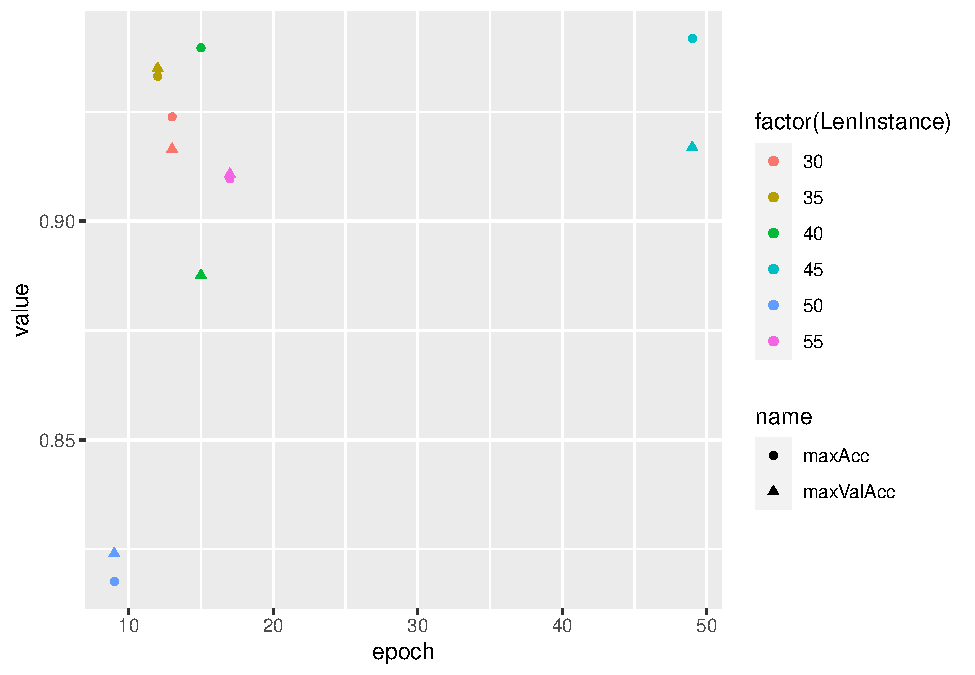
\includegraphics{CAMS-Project-Progress_files/figure-latex/unnamed-chunk-4-1.pdf}

\hypertarget{performance}{%
\chapter{Model Performance}\label{performance}}

\begin{Shaded}
\begin{Highlighting}[]
\FunctionTok{library}\NormalTok{(tidyverse)}
\end{Highlighting}
\end{Shaded}

\begin{Shaded}
\begin{Highlighting}[]
\NormalTok{featureset\_df }\OtherTok{=} \FunctionTok{read\_csv}\NormalTok{(}\StringTok{\textquotesingle{}data/featuresets\_ModelHistories.csv\textquotesingle{}}\NormalTok{)}

\NormalTok{accuracy\_df }\OtherTok{\textless{}{-}}\NormalTok{ featureset\_df }\SpecialCharTok{\%\textgreater{}\%}
  \FunctionTok{rename}\NormalTok{(}\AttributeTok{train\_loss =}\NormalTok{ loss, }\AttributeTok{train\_accuracy =}\NormalTok{ accuracy) }\SpecialCharTok{\%\textgreater{}\%}
  \FunctionTok{select}\NormalTok{(}\SpecialCharTok{{-}}\FunctionTok{c}\NormalTok{(}\StringTok{"val\_loss"}\NormalTok{, }\StringTok{"train\_loss"}\NormalTok{)) }\SpecialCharTok{\%\textgreater{}\%}
  \FunctionTok{pivot\_longer}\NormalTok{(}\AttributeTok{cols =} \FunctionTok{c}\NormalTok{(train\_accuracy, val\_accuracy), }\AttributeTok{names\_to =} \StringTok{"phase"}\NormalTok{, }\AttributeTok{values\_to =} \StringTok{"accuracy"}\NormalTok{)}

\NormalTok{loss\_df }\OtherTok{\textless{}{-}}\NormalTok{ featureset\_df }\SpecialCharTok{\%\textgreater{}\%}
  \FunctionTok{rename}\NormalTok{(}\AttributeTok{train\_loss =}\NormalTok{ loss, }\AttributeTok{train\_accuracy =}\NormalTok{ accuracy) }\SpecialCharTok{\%\textgreater{}\%}
  \FunctionTok{select}\NormalTok{(}\SpecialCharTok{{-}}\FunctionTok{c}\NormalTok{(}\StringTok{"val\_accuracy"}\NormalTok{, }\StringTok{"train\_accuracy"}\NormalTok{)) }\SpecialCharTok{\%\textgreater{}\%}
  \FunctionTok{pivot\_longer}\NormalTok{(}\AttributeTok{cols =} \FunctionTok{c}\NormalTok{(train\_loss, val\_loss), }\AttributeTok{names\_to =} \StringTok{"phase"}\NormalTok{, }\AttributeTok{values\_to =} \StringTok{"loss"}\NormalTok{)}
\end{Highlighting}
\end{Shaded}

\begin{Shaded}
\begin{Highlighting}[]
\FunctionTok{ggplot}\NormalTok{(accuracy\_df, }\FunctionTok{aes}\NormalTok{(}\AttributeTok{x =}\NormalTok{ epoch, }\AttributeTok{y =}\NormalTok{ accuracy, }\AttributeTok{color =}\NormalTok{ variable\_set, }\AttributeTok{linetype =}\NormalTok{ phase)) }\SpecialCharTok{+} 
  \FunctionTok{geom\_line}\NormalTok{(}\AttributeTok{linewidth =} \DecValTok{10}\NormalTok{) }\SpecialCharTok{+} 
  \FunctionTok{ylim}\NormalTok{(}\FloatTok{0.4}\NormalTok{,}\FloatTok{1.0}\NormalTok{) }\SpecialCharTok{+}
  \FunctionTok{facet\_grid}\NormalTok{(}\FunctionTok{vars}\NormalTok{(model), }\FunctionTok{vars}\NormalTok{(len\_instance)) }\SpecialCharTok{+}
  \FunctionTok{ggtitle}\NormalTok{(}\StringTok{"Model Training History Comparison"}\NormalTok{, }\AttributeTok{subtitle =} \StringTok{"Differences between training and test performance across feature sets."}\NormalTok{) }\SpecialCharTok{+} \FunctionTok{theme}\NormalTok{(}\AttributeTok{legend.position =} \StringTok{"bottom"}\NormalTok{)}
\end{Highlighting}
\end{Shaded}

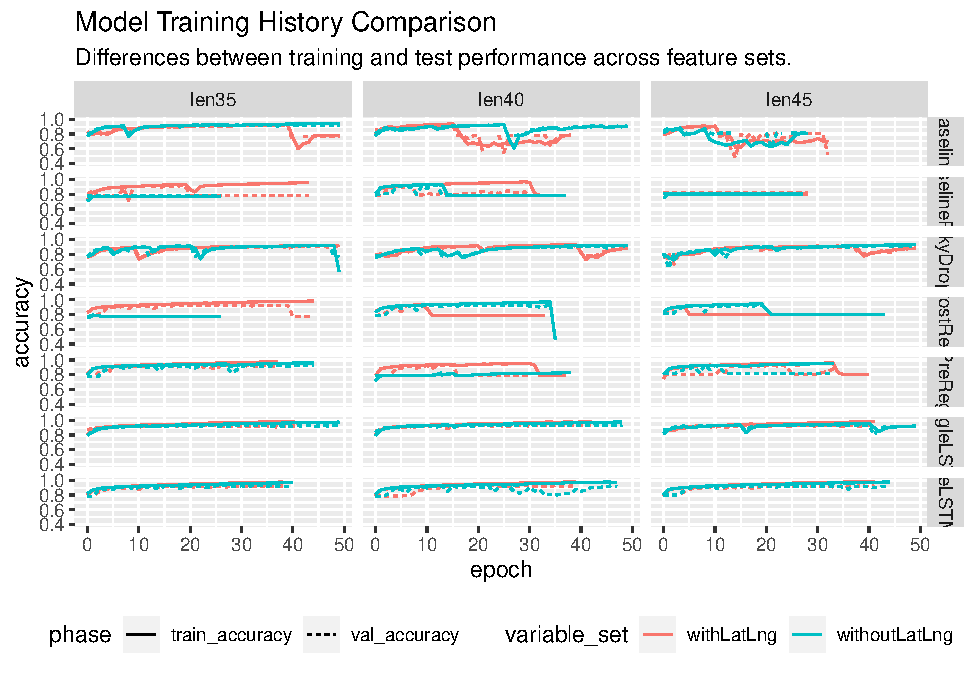
\includegraphics{CAMS-Project-Progress_files/figure-latex/unnamed-chunk-7-1.pdf}

  \bibliography{book.bib,packages.bib}

\end{document}
